\chapter{Optimization and Control of a kHz Laser System} \label{ch:6}

The work of \autoref{ch:5} has illustrated the usefulness of machine learning methods in the field of ion acceleration and what sort of quantities might be optimized. To generate enough data for the \gls{ML} algorithms, the facilities need to use both a high-repetition rate laser (i.e. many shots per second) and a continuously refreshing target (e.g. a flowing liquid or tape drive target). Using such a system, no research group has yet obtained a stable and tunable MeV source of protons required for applications. Using a solid Kapton tape, Loughran et al. \cite{Loughran_2023_HPLSE} used \gls{BO} at \gls{RAL}, but only on around 60 bursts of shots. Using a flowing liquid target, multi-MeV deuteron acceleration \cite{Treffert_2022_APL} was demonstrated from a flowing liquid target at \gls{CSU}, but only operated over 2 minutes for a total of 60 shots.

At the Wright-Patterson Air Force Base, a 1 kHz, mJ class laser system exists that is capable of producing MeV protons \cite{Morrison_2018_NJoP}. In comparison to the two previously mentioned studies at \gls{CSU} and \gls{RAL}, a 1 kHz laser shoots one thousand to two thousand times more shots per second! A laser system that shoots one thousand times more shots per second, however, will also roughly have a thousand times less laser energy per shot. Morrison et al. \cite{Morrison_2018_NJoP} was able to achieve 2 MeV protons on this kHz system at \gls{WP-ELL}, while higher energy Hz laser systems can easily achieve tens of MeV. 

To enhance the MeV proton yield within the existing mJ class laser system, the \gls{TNSA} mechanism needs to be optimized as much as possible. This can be done in multiple ways:

\begin{itemize}
\item As explained in \autoref{ch:4}, multiple pulses can yield higher proton energies with the same amount of laser energy through \gls{eTNSA}. Even when the pulses are not spatially aligned, the preplasma induced from the first pulse can enhance the absorption in from the second pulse and yield higher proton energies as long as the rear side of the target is relatively undisturbed \cite{Macchi_2013_RevModPhys}. Relevant parameters here would be pre-pulse contrast, time delay between pulses, and a variety of other spectral properties of the pulse could even be optimized through the use of an instrument like the DAZZLER (see Loughran et al. \cite{Loughran_2023_HPLSE} for an example). 

\item Generally, thinner targets see enhanced proton acceleration via the vacuum heating mechanism which is a well known scaling captured in the Fuchs et al. \cite{Fuchs_2005_Nat} model explored in \autoref{ch:5}. However, targets that are too thin may break up before the acceleration takes place. Relevant parameters here would be the thickness, composition, and shape of the target. 
\end{itemize}
Evidently, many parameters influence the laser-target interaction in a very non-linear way which cannot be easily seen through the raw data. In this chapter, I give an overview of the kHz laser system at \gls{WP-ELL} and particularly focus on the \gls{DAQ} developed by fellow graduate student Nathaniel Tamminga and \gls{CSUCI} professor Scott Feister. Then, the code and machine learning framework that I developed, with some help from Jack Felice, to send optimized parameters back to the \gls{DAQ} is described. Finally, some results from this elementary machine learning feedback loop are discussed. The experimental operation of the laser was handled by the lab technician Kyle Frische. Miami University professor and former OSU graduate student Joseph Snyder helped with the experiments using his prior experience at the laboratory. Additionally, Anil Patnaik and Michael Dexter from AFIT and OSU professor Enam Chowdhury gave valuable feedback during weekly meetings for this effort. The results from this work are currently under consideration at \emph{APL Machine Learning}.

\section{Background} \label{sec:lab_background}

In this section, I will describe the experimental setup at the \gls{WP-ELL} which uses a Ti:Sapphire based ultra-intense $780 \unit{\nano \meter}$ laser and a liquid sheet target.  

\subsection{Experimental Chamber}

With a maximum energy of $\sim 9 \unit{mJ}$, \gls{FWHM} period of $35 \unit{\femto \second}$, the \gls{WP-ELL} laser system is capable of producing pulses of peak intensity $\SI{5e18}{\watt \per \centi \meter \squared}$ with a 1.8 $\unit{\micro \meter}$ \gls{FWHM} spot size. By picking off a small amount of laser energy from the main pulse ($\sim \SI{12}{\micro \joule}$), an artificial pre-pulse can be used with a tunable delay between the pulses. Each of the beams are focused by an \gls{OAP}. These features are shown in \autoref{fig:experimental_chamber}. Additionally, a sequence of waveplates allows the main pulse and pre-pulse intensity to be reduced by up to a factor of ten by simply rotating the plate to a precise angle.

\begin{figure}
	\centering 
	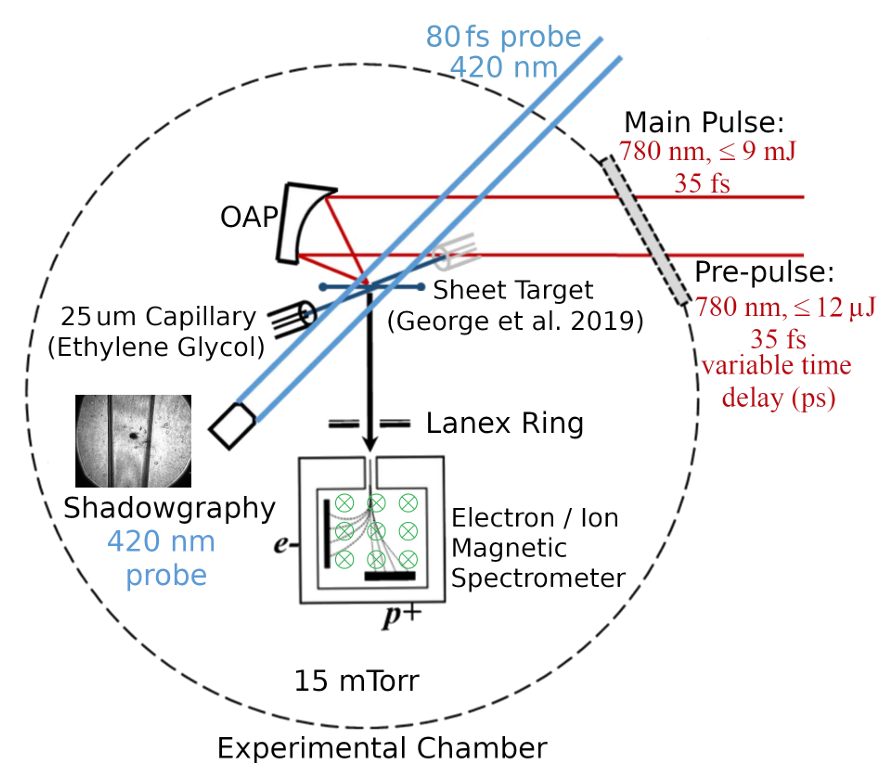
\includegraphics[width=0.75\linewidth]{planning/images/daq/experimental_chamber.PNG}
	\caption{A schematic of the experimental chamber, targetry system, diagnostics, and laser pulses entering the chamber at a kHz repetition rate. Figure taken from a manuscript in review by Tamminga et al.}
	\label{fig:experimental_chamber}
\end{figure}

The sheet target, described in detail in George et al. \cite{George_2019_HPLSE}, is formed by the grazing incidence of two extremely thin liquid stream of around 25 $\unit{\micro \meter}$ each. The target can be seen via shadowgraphy as seen in \autoref{fig:liquid_leaf}(A). The laser interaction with the sheet target can be seen in \autoref{fig:experimental_chamber} as the black dot in the center of the shadowgraph. We can see in \autoref{fig:liquid_leaf}(B) that the target has an oval shape which is why it is sometimes referred to as a ``liquid-leaf'' target \cite{Schmitz_2023_LaPB}. Since background particles are deleterious to the laser-matter interaction \cite{Snyder_2020_SciRep}, the chamber is pumped down to a pressure of 15 mTorr. Ethylene glycol is the chosen liquid in this experiment due to its ability to exist as a liquid at room temperature at these extremely low vacuum pressures, but other liquids (like $\text{H}_2\text{O}$ or $\text{D}_2\text{O}$) can be used as well at a possibly higher pressure.

\begin{figure}
	\centering 
	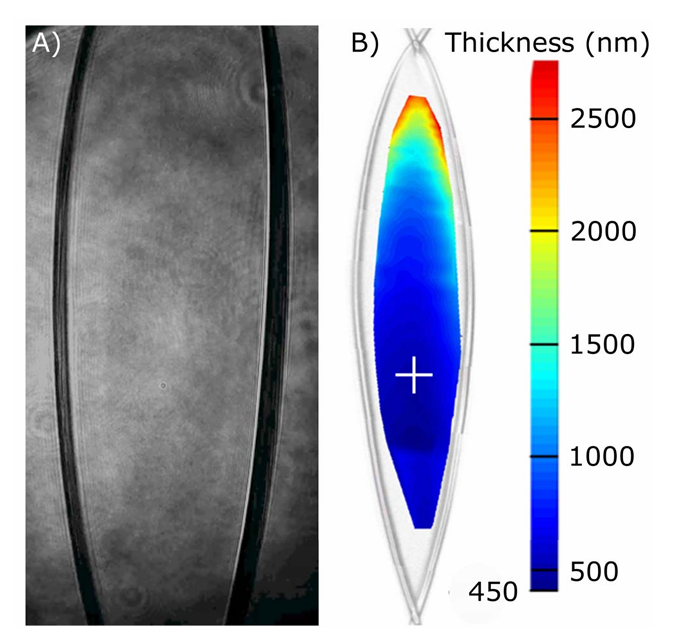
\includegraphics[width=0.75\linewidth]{planning/images/daq/target.PNG}
	\caption{(A) Microscope Shadowgraphy image of the central region of the liquid sheet target in vacuum. (B) Spatially dependent thickness map across the liquid sheet, collected with a Filmetrics white-light interference profiler. The white cross indicates the location of the minimum sheet thickness at 450 $\unit{\nano \meter}$. For scale, the width of the sheet in (B) is 560 $\unit{\micro \meter}$. A schematic of the experimental chamber, targetry system, diagnostics, and laser pulses entering the chamber at a kHz repetition rate. Figure reprinted from Figure 5 of George et al. \cite{George_2019_HPLSE}.}
	\label{fig:liquid_leaf}
\end{figure}

The electrons and ions accelerated normal to the rear of the sheet target travel through a Lanex Ring into the magnetic spectrometer. This spectrometer uses a magnet that deflects negative particles to the left and positive particles to the right (in reference to \autoref{fig:experimental_chamber}). Using the fact that the cyclotron radius of a charged particle in a magnetic field varies based on its velocity, the final location of the deflected particle determines its kinetic energy. The \gls{CCD} detectors are coated with scintillating material which converts the particle energy into a light signal that the \gls{CCD}s are capable of detecting.  

\subsection{Data Sources} \label{sec:data_sources}
\subsubsection{Spectrometers}

The electron and proton spectra are collected from Mightex \gls{CCD} cameras and stored in \gls{HDF5} files. They each have 3648 pixels with $\SI{8}{\micro \meter}$ pixel width. As can be seen from \autoref{fig:experimental_chamber}, the higher energy particles should be reflected less and should (which translates to hitting the right end of the detector for electrons and the left end of the detector for positive ions). The magnetic field profile has been mapped out in previous work \cite{Morrison_2018_NJoP} so that a one-to-one correspondence between pixel location and kinetic energy can be established for both electrons and protons seen in \autoref{fig:pixel_energy}. 

The CCD pixels store counts up to 65,536 (unsigned 16 bit integer) which are collected over the desired exposure time. For example, if the Mightex cameras are set to collect at 100 Hz, they can have an exposure time of up to 10 ms. Pixels 0 to 900 for the proton CCD fall close to the direct line of sight of an undeflected particle and thus can receive stray signals from other radiation sources like x-rays. Since protons from this laser system have peaked at 2.5 MeV \cite{Morrison_2018_NJoP} (around pixel 1000), ignoring pixels 0 to 900 does not throw away any high energy proton data. Furthermore, 13 (additional) pixels are shielded from light which can be used to set a noise floor.

\begin{figure}
	\centering 
	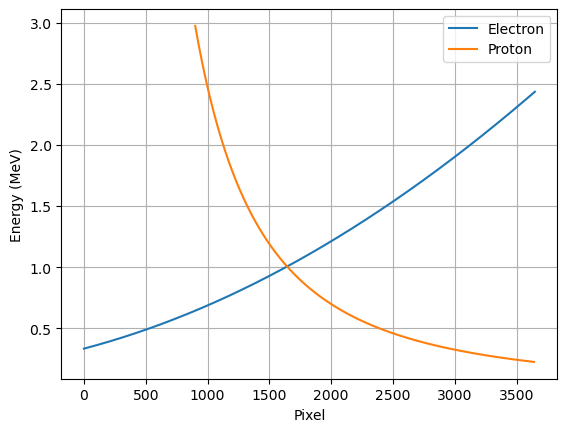
\includegraphics[width=0.75\linewidth]{planning/images/daq/pixel.png}
	\caption{The pixel number to proton or electron kinetic energy mapping for the two \gls{CCD}s present in the magnetic spectrometer. This is the same mapping that was used in Morrison et al. \cite{Morrison_2018_NJoP}.}
	\label{fig:pixel_energy}
\end{figure}

\subsubsection{Laser Diagnostics}
To accurately measure the main pulse and pre-pulse energy (or intensity) at a kHz rate, a tiny fixed percentage of the pulses are picked off and redirected at a diode. This diode measures a momentary increase in voltage over the course of 1 ms (due to the kHz collection rate) shown in \autoref{fig:diode_trace}. The peak of this trace will be directly proportional to the energy of an individual shot. \autoref{fig:diode_peak} shows this voltage plotted over a range of 30,000 shots (30 seconds) where the laser energy was increased and decreased.

\begin{figure}
	\centering 
	\subfloat{
		\label{fig:diode_trace}
		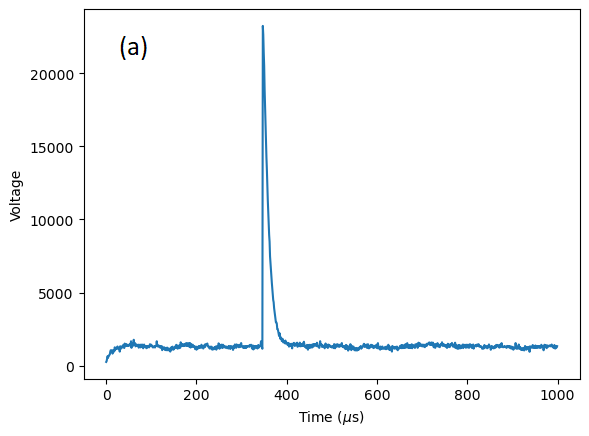
\includegraphics[width=0.5\linewidth]{planning/images/daq/diode_trace.png}
	}
	\subfloat{
		\label{fig:diode_peak}
		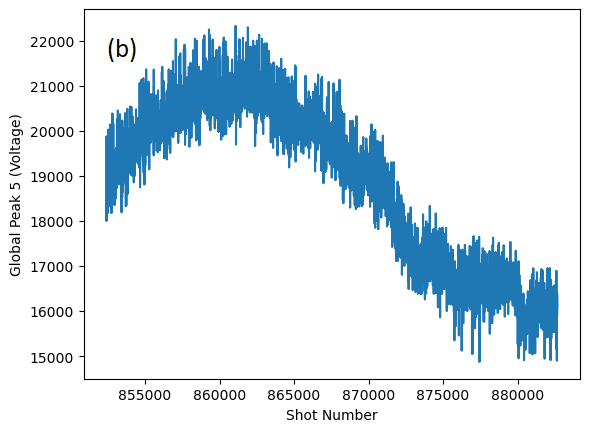
\includegraphics[width=0.5\linewidth]{planning/images/daq/diode_peak.png}
	}
	\caption{(a) An example of the voltage trace each individual shot registers on the laser diode. (b) The peak of the voltage trace is plotted for a range of shots.}
\end{figure}

The calibration between the peak voltage and laser energy is shown in \autoref{fig:energy_calibration} which is clearly a linear relationship for both main and pre-pulse. As mentioned earlier, the angle of two polarizing waveplates controls the amount of energy that strikes the target. These two angles are tunable and can be accurately fit to the energy by using Malus' Law ($I = I_0 \cos^2(\theta)$).

\begin{figure}
	\centering 
	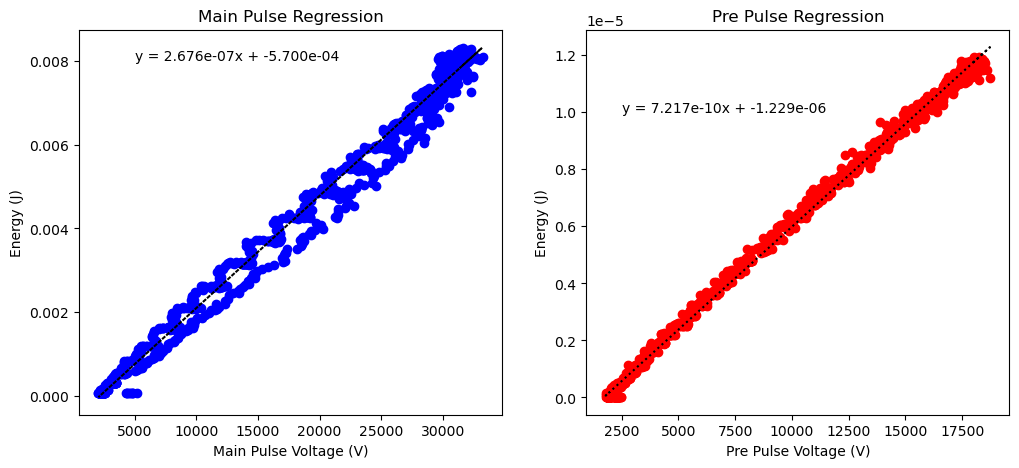
\includegraphics[width=0.9\linewidth]{planning/images/daq/energy_calibration.png}
	\caption{Linear relation from voltage to energy for both the main pulse (blue) and pre-pulse (red). The slope and intercept are displayed on the graphs.}
	\label{fig:energy_calibration}
\end{figure}

\subsubsection{Target Properties}

As seen in \autoref{fig:experimental_chamber}, the sheet target is created by the interaction of two grazing incidence liquid microjets that shoot from two nozzles. These  are situated on an XPS motion controller whose orientation and position can be precisely tuned to micron-level precision. 

In this work, we change the target position along the laser-axis direction which changes the distance between the peak focus of the laser and the target. However, the XPS controllers have the ability to control other properties. The vertical target position can be changed which can, in principle, alter the target thickness as shown in \autoref{fig:liquid_leaf}(B). Additionally, the nozzle angles and positions could be adjusted to modify the target shape. Like the \gls{CCD}s and diodes, the target data is also stored in the \gls{HDF5} format (currently at a 5 Hz rate).

\subsubsection{Other Sources}
There are other potential radiation sources that can be measured but I will give two others as examples. The amount of ionizing radiation is already recorded the \emph{Radiation Survey Log} that AFIT graduate student Benjamin Knight has created in units of mR/h (milli roentgen per hour). Second, neutrons have been detected \cite{Knight_2024_HPLSE} and optimizing their counts could give insights into high-repetition rate fusion.

\section{Optimization Experiments} \label{sec:daq_results}

In this section, the data analysis suite that I have developed will be explained in detail. Then, some results from one highlighted day will be explored to demonstrate the types of experiments that one could conduct using this setup.

\subsection{Automated Data Extraction}

\subsubsection{Combining Data}

Nathaniel and Scott have spent a great deal of time, before my involvement in the project, in making sure all the data sources described in \autoref{sec:data_sources} are accurately synced up on a common index: the shot count. They have successfully integrated the lab with \gls{EPICS} which allows the values of the aforementioned data sources to be broadcasted throughout the lab network. In this way, we can extract the values of the waveplate angles, target positions, pre-pulse delay, and other values from any of the computers in the lab at any time. Furthermore, we can use \gls{EPICS} commands from python scripts, LabVIEW interfaces, and other means to adjust these parameters in real time. Below, I will describe the process that I used to combine all the data and perform the analysis. 

To start, I looked at the relevant locations at the lab computers to automatically grab the files from all the relevant data sources within a given time window (most of which were stored as \gls{HDF5} files). I then created a pandas dataframe where each point corresponds to a unique Mightex shot count (i.e. an individual data point on the spectrometers). So, if the spectrometers were collecting at 20 Hz, I would take a rolling average of 50 nearby shots to compress the 1 kHz main and pre-pulse data down to 20 Hz. On the other hand, the target position and delay time were interpolated to fill values at a 20 Hz rate (since they collected at a 5 and 2 Hz rate respectively).

Then, to smooth the spectra, I subtracted out the noise using counts from the light shielded pixels and applied a median filter of window size 15 (replaces the given pixel counts with the median of the adjacent 15 pixel counts). From the spectra data, I extracted two metrics: the 99th percentile energy/pixel $E_\text{max}$ and the total \gls{CCD} counts $N$. Furthermore, I provided some extra processing to improve the data quality. First, I threw out data points that were oversaturated -- that is the counts were so high that they were getting maxed out (beyond unsigned 16 bit precision) for a given pixel. Second, I removed points that didn't contain a sufficient number of electron or proton counts. Third, I implemented a measure to catch and fix the shot count if one of the spectrometers temporarily froze and reset its internal shot count. 

Finally, I merged all the data sources together in one pandas dataframe which was then saved to a compressed \gls{HDF5} file.

\subsubsection{Data Visualization}
Given a merged and filtered dataset, visualizing the data is easy (see \autoref{fig:optimization_gui}) which is based on data collected on June 14th 2024. In \autoref{fig:optimization_gui}(B), the main pulse and pre-pulse parameter space is adequately explored over a 45 minute time frame. In \autoref{fig:optimization_gui}(C), the cosine-squared mapping between the waveplate angle and diode voltage for both main and pre-pulse is shown. In the lab, the angle of the main pulse waveplate drifts over time, so an initial angle ``$\theta_0$'' is automatically inferred from the data corresponding to the waveplate angle that registers maximum voltage. In \autoref{fig:optimization_gui}(D), the main pulse and target focus position (\texttt{nozzle\_focus}) are plotted as a function of shot number (and time) which shows approximately 25,000 shots worth of data.

\begin{figure}
	\centering 
	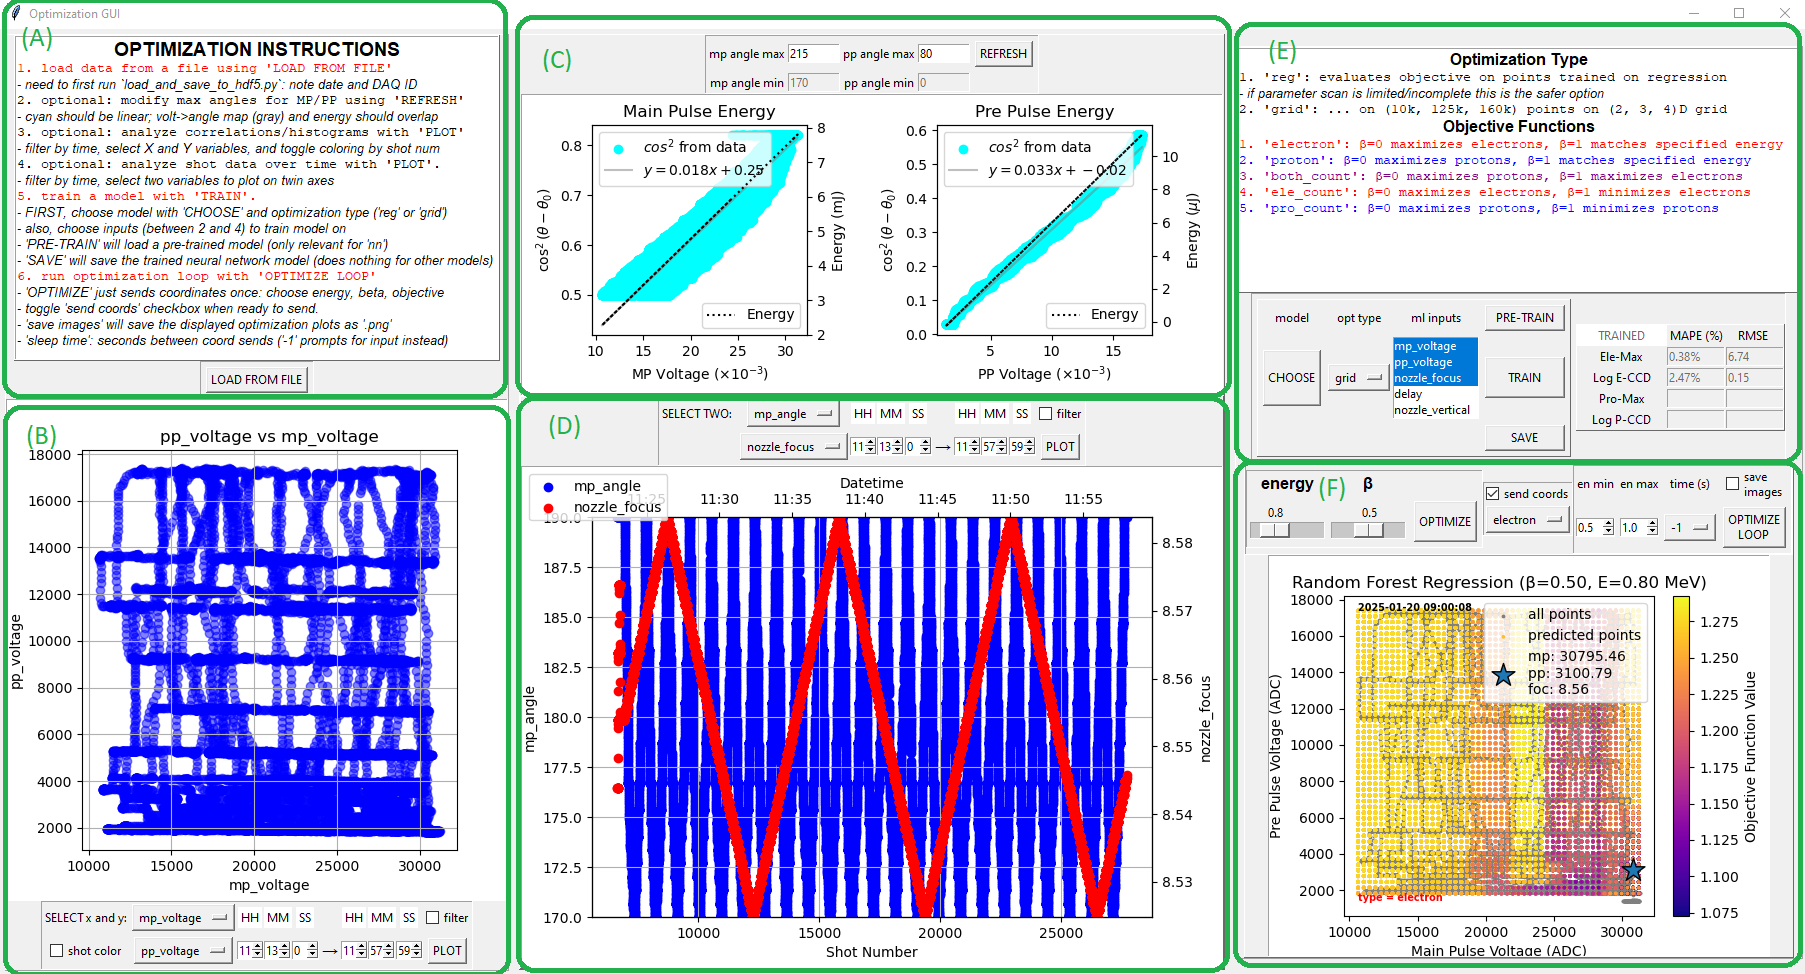
\includegraphics[width=\linewidth]{planning/images/daq/optimization_gui.png}
	\caption{(A) A list of instruction on how to use the \gls{GUI} and a button that loads in data already saved to a compressed \gls{HDF5} file. (B) A panel that shows two variables plotted against each other. (C) The mapping between cosine-squared of the waveplate angle and the measured voltage on the laser diodes. (D) Two variables are plotted as a function of time and shot number. (E) Instructions for the optimization task with options to choose a machine learning model, desired inputs, and displayed error metrics after training the model. (F) A visual of the optimization task which shows darker purple colors in regions of the parameter space that best optimize the chosen metric from \autoref{eq:obj_function_daq}.}
	\label{fig:optimization_gui}
\end{figure}

To visualize the electron/proton spectrum, I used a different \gls{GUI} which first loads data from a file shown in \autoref{fig:spectrum_gui}(A). In \autoref{fig:spectrum_gui}(B), the spectrum is plotted throughout the run and the bright yellow spots correspond to shot numbers and pixels with high counts. In \autoref{fig:spectrum_gui}(C), a diagnostic plot is shown that measures the number of skipped shots in the data. Sometimes, especially when running the spectrometers at a higher repetition rate, shots can be skipped over due to the inability of the virtual machines to keep up with the data acquisition. In \autoref{fig:spectrum_gui}(D, E) the electron spectrum for a specified shot is plotted as a function of either pixel number of energy in MeV. These can either be plotted on a linear y-scale or a log y-scale.

\begin{figure}
	\centering 
	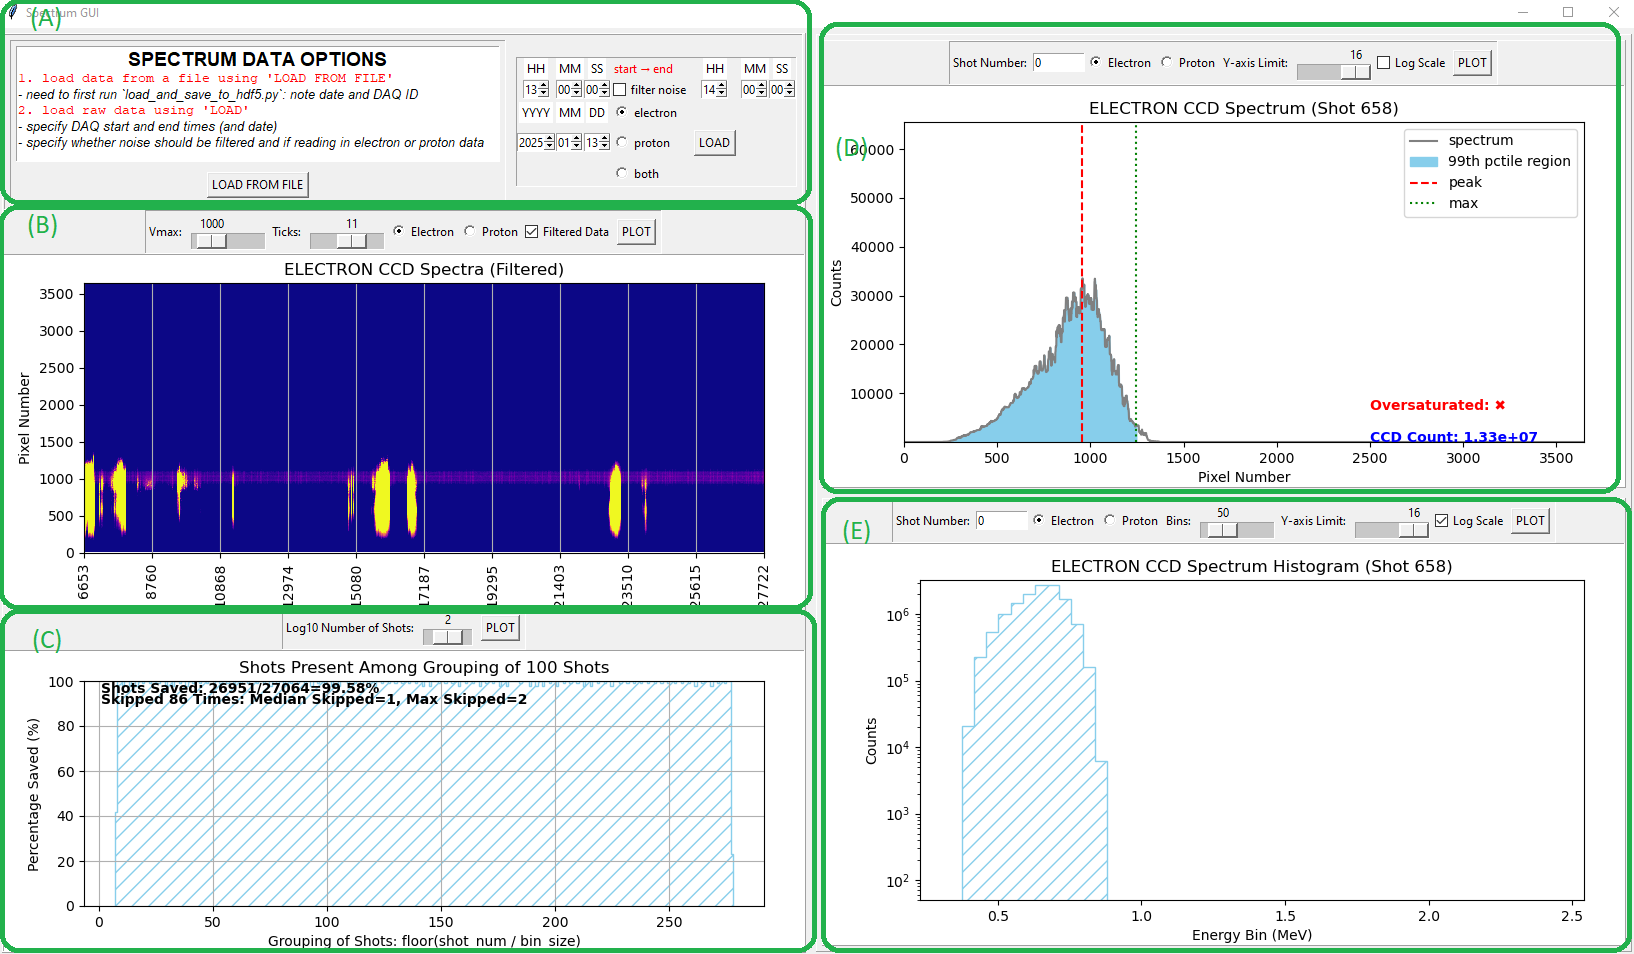
\includegraphics[width=\linewidth]{planning/images/daq/spectrum_gui.png}
	\caption{(A) A list of instructions on how to load in the data. (B) A heatmap that shows the pixel counts for the shot numbers throughout the run. (C) A diagnostic that shows where (if any) shots are erroneously being missed due the lab equipment. (D) An electron spectrum plotted for a specified shot. (E) An electron spectrum binned by energy in MeV on a log scale.}
	\label{fig:spectrum_gui}
\end{figure}

\subsection{Optimization Feedback Loop}
The developed \gls{ML} framework was tested out on various days in the summer of 2024. In this subsection, I will highlight one particular day: June 14th, 2024 which varied the main-pulse, pre-pulse and target position according to \autoref{tab:exp_runs}. The data seen in \autoref{fig:optimization_gui} and \autoref{fig:spectrum_gui} are also from this day. 


\begin{table}
	\centering
	\begin{tabular}{|p{4cm}|p{1.5cm}|p{1.5cm}|p{3cm}|}
		\hline
		\textbf{Explored Parameter} & \text{Max} & \textbf{Min} & \textbf{Scan Period}\\
		\hline
		Main Pulse Energy & 8.4~mJ & $\lesssim$1~mJ & 80 s\\
		\hline
		Pre-Pulse Energy & 12~$\mu$J & $\lesssim$1~$\mu$J & 104 s\\
		\hline
		Target Position & +30~$\mu$m & -30~$\mu$m & 700 s\\
		\hline
	\end{tabular}
	\caption{A description of the experimental parameters, the range they were scanned through, and the period of the parameter scan. This table was reproduced from forthcoming work in Tamminga et al. (2025).}
	\label{tab:exp_runs}
\end{table}

These three quantities were simultaneously varied with three different periods so that the 3D parameter space would be adequately explored. The approximately 25,000 data points from this 45 second run were stored in a consolidated \gls{HDF5} file. After this, we used the optimization \gls{GUI} in \autoref{fig:optimization_gui}(E) to quickly fit a regression with specified hyperparameters on the collected data. Similar to \autoref{sec:second_analysis}, we used min-max scaling on all the inputs due to the fixed parameter bounds in \autoref{tab:exp_runs}, but use standard z-score scaling on the outputs (logarithm of the ccd counts and 99th percentile energy). This model is used to smooth over noisy data points and we can apply a metric (just like what was done in \autoref{sec:first_analysis} and \autoref{sec:second_analysis}) to optimize for two different properties. Here, we use the following objective function

\begin{equation}
	f(KE_{\rm cutoff},N_{e})  =  1 + (1 - \beta) \cdot \left(1 -  \frac{\log_{10}(N_{e})}{8} \right) + \beta \frac{|KE_{\rm c} - KE_{\rm c,goal}|}{KE_{\rm c, goal}} \label{eq:obj_function_daq}
\end{equation}
which looks notably similar to \autoref{eq:obj_function_v2} if the logarithm of the \gls{CCD} electron counts $N_e$ replaces the conversion efficiency $\eta$. We attempted to perform a similar optimization task as explored in \autoref{ch:5}, but the electron data largely had signals at the same energy which can be seen in \autoref{fig:spectrum_gui}(D, E). This spectrum peaks around 0.7 or 0.8 MeV but can have a higher or lower number of counts based on the input parameters. We found (unsurprisingly) that the conditions with highest electron counts correspond to maximum main pulse intensity, minimum pre-pulse intensity, and close to peak focus. An example of this can be seen in \autoref{fig:optimization_gui}(F) which highlights the main pulse and pre-pulse optimal conditions with a blue star. For this run, 8.555 mm was the absolute position of the target when peak focus was achieved which matches the peak focus listed in the figure legend.

Even though the electron spectra did not offer a lot of interesting physics to explore, we did successfully implement a feedback loop which sent the optimized main pulse, pre-pulse, and focus conditions back to motion controllers and waveplates in the lab via the \gls{EPICS} protocol. An example of this can be seen in \autoref{fig:beta_shift} where, during a second data collection, optimized parameters from the first run were sent via \gls{EPICS} to change the electron spectra in real-time. Each value of $\beta$ specified a slightly different set of input parameters that were tested for 30 seconds before moving on to the next value of $\beta$. We can see that the higher values of $\beta$ have maximum electron kinetic energy closer to 0.7 MeV in comparison to the lower values of $\beta$ (with the notable exception $\beta=0$). Importantly, these steps were all taken automatically through the use of a Python script.

\begin{figure}
	\centering 
	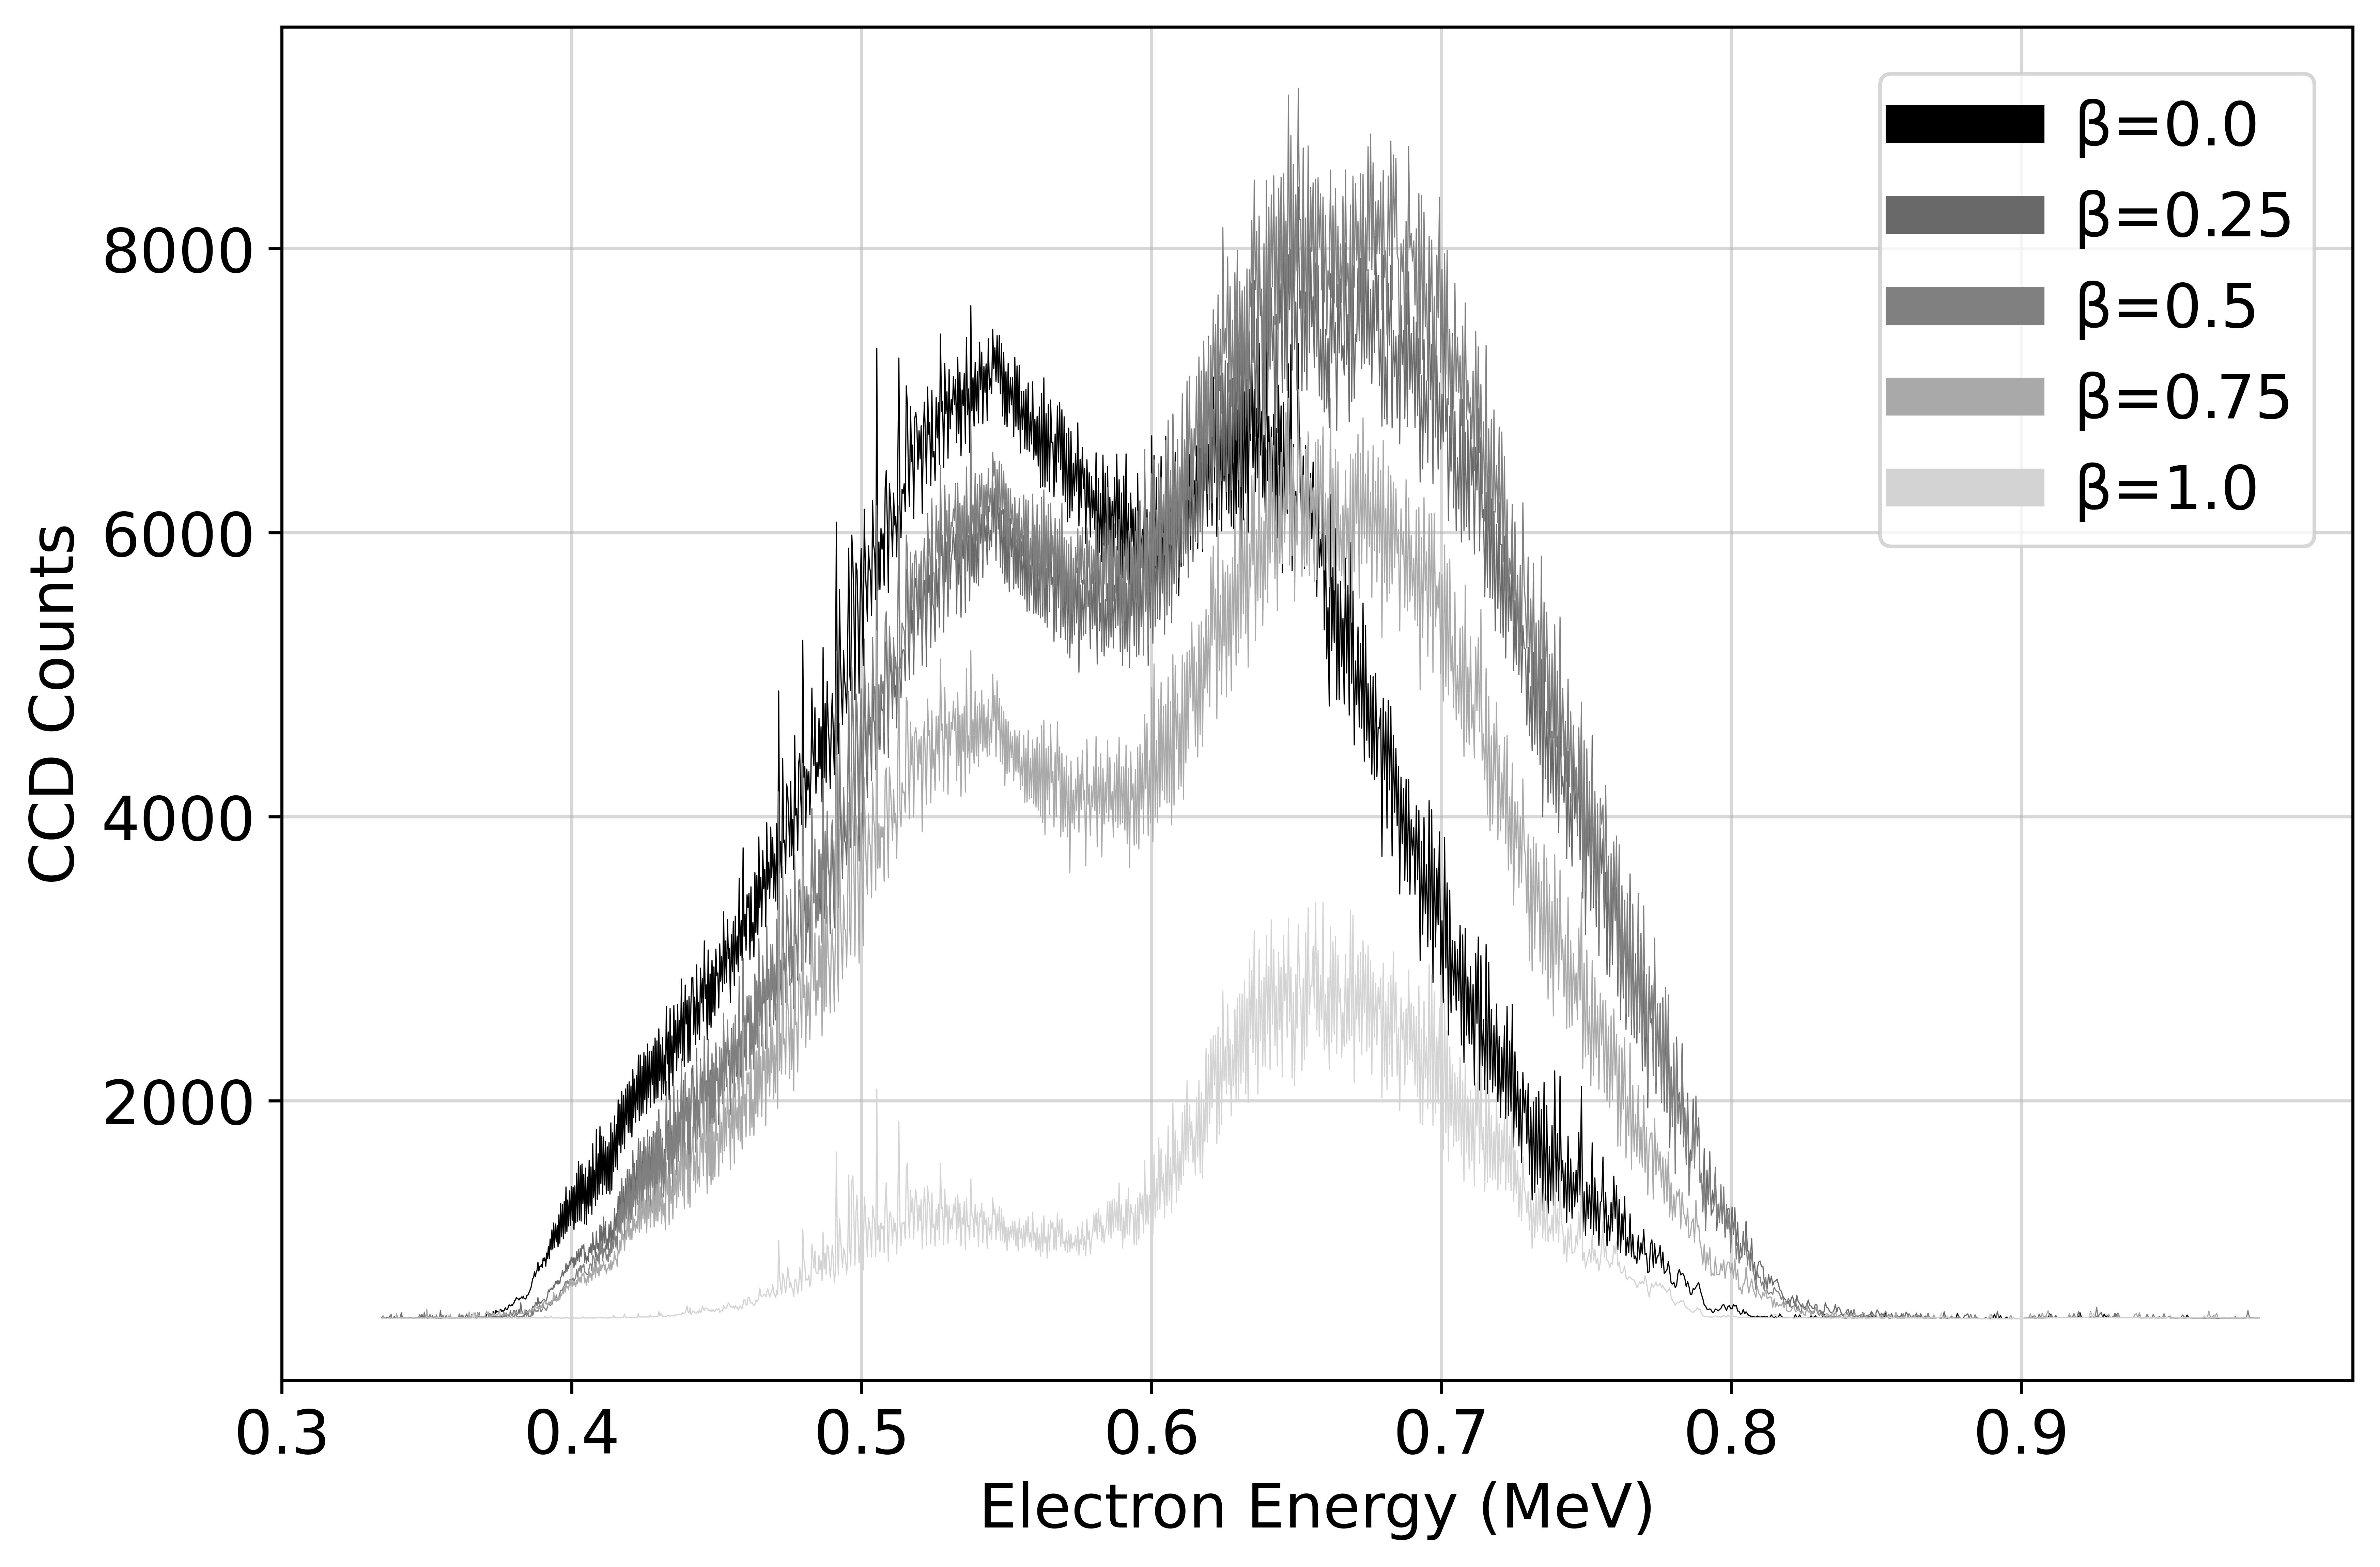
\includegraphics[width=0.6\linewidth]{planning/images/daq/rf_beta_shift.jpg}
	\caption{Electron spectra plotted for various levels of $\beta$ for a specified cutoff energy $KE_{\rm c,goal} = 0.7$ MeV. The different spectra are predicted optimal parameters from a \gls{RFR} model trained on data collected in an earlier run.}
	\label{fig:beta_shift}
\end{figure}

\section{Conclusion}

The chapter started by overviewing the experimental setup in \autoref{sec:lab_background} of the \gls{WP-ELL} which includes a 1 kHz femtosecond laser, up to 100 Hz particle spectrometers, and a free-flowing liquid target. Many parameters like the main/pre-pulse peak intensity, focus position in reference to the target, pulse delays, and more can be easily adjusted manually with the click of a button. Then, we explained the optimization experiment in \autoref{sec:daq_results} that involved collecting data from one run where three input parameters were varied simultaneously. This data was used to train a \gls{ML} model that could map these three input target conditions to features of an electronic spectra: the maximum energy and total counts on the \gls{CCD}. The trained model was then used to predict optimal inputs according to \autoref{eq:obj_function_daq}). Finally, these predicted optima were sent via \gls{EPICS} to the relevant lab equipment in an automated way to explore laser and target conditions that yield a desired spectrum. We showed in \autoref{fig:beta_shift} that this feedback loop can work in principle to balance two competing properties: maximum kinetic energy and high electron counts. 

While this work is certainly important, it is still in early stages. We have the ability to collect proton spectra which can be more difficult to obtain but have more use for applications. However, the amount of proton data that we are able to get is usually minimal -- much of the explored parameter spaces end up with no proton signal. To make real progress, we would need to make improvements on the experimental side to obtain a more stable target that could more reliably generate MeV protons for a range of different input conditions.

Furthermore, our current feedback loop involves fitting a relatively simple regression to the data -- something that is only possible when the size of the data is small (tens of thousands) and there are only a few different parameters. A more useful model that could feasibly handle larger and more complex datasets would be the \gls{NN} as evidenced by \autoref{sec:second_analysis}. Additionally, \gls{GPU}-accelerated computations would be necessary to operate this feedback loop in real-time. After obtaining several high-quality datasets scanning different parameters, we could pre-train the \gls{NN} so that when presented with a limited amount of new data from a different day, it could more quickly assess the ideal laser conditions. Nonetheless, the work presented here represents an important first step in incorporating \gls{ML} methods to optimize \gls{TNSA} accelerated protons in real-time. 